\section{Dijet Production}
\label{sec:Theory:Dijet}

The main analysis of this thesis is directed towards dijet production with a veto on additional jet radiation between the dijets.
Dijet production cross-section can be calculated using Equation \ref{Theory:XSec} with the $\hat{\sigma}$ being the partonic cross-section for $2\rightarrow 2$ scattering.
Measured dijet production cross-sections as a function of the dijet kinematics, for instance the dijet mass, can be compared to leading order (LO) and next-to-leading order (NLO) cross-section calculations.
The dijet cross-section measured by the ATLAS Collaboration is compared to NLO cross-section calculation in \cite{ref:Dijet}, with an agreement within the experimental uncertainty.
LO cross-section calculations have the lowest order of $\alpha_{s}$ needed to get the correct final state, for dijets this is $\alpha_{s}^{2}$.
Some of the LO parton scattering diagrams are shown in Figure \ref{Theory:LODijet}.
Next-to-leading order (NLO) cross-section calculations consist of the LO cross-sections with $\alpha_{s}^{2}$, plus the next order in the perturbative series expanded in $\alpha_{s}$, i.e. $\alpha_{s}^{3}$.
       \unitlength = 1mm
\begin{figure}
\centering
\mbox{
     
\begin{fmffile}{figures/QCD/gg1}
\begin{fmfgraph}(40,25)
\fmfleft{i1,i2}
\fmfright{o1,o2}
\fmf{gluon}{i1,v1,o1}
\fmf{gluon}{i2,v2,o2}
\fmf{gluon}{v1,v2}
\end{fmfgraph}
\end{fmffile}


\begin{fmffile}{figures/QCD/gg2}
\begin{fmfgraph}(40,25)
\fmfleft{i1,i2}
\fmfright{o1,o2}
\fmf{gluon}{i1,v1,o1}
\fmf{gluon}{i2,v1,o2}
\end{fmfgraph}
\end{fmffile}
     
     
    

\begin{fmffile}{figures/QCD/gg3}
\begin{fmfgraph}(40,25)
\fmfleft{i1,i2}
\fmfright{o1,o2}
\fmf{gluon}{i1,v1,i2}
\fmf{gluon}{o1,v2,o2}
\fmf{gluon}{v1,v2}
\end{fmfgraph}
\end{fmffile}

}

\enskip

\mbox{
 
   
%    Hello
%    
%\begin{fmffile}{gg4}
%\begin{fmfgraph}(40,25)
%\fmfleft{i1,i2}
%\fmfright{o1,o2}
%\fmf{phantom,tension=1.5}{i1,v1}
%\fmf{phantom,tension=1.5}{i2,v2}
%\fmf{phantom}{i1,v1,o1}
%\fmf{phantom}{i2,v2,o2}
%\fmf{gluon,tension=0}{i1,v1,o2}
%\fmf{gluon,tension=0,rubout}{i2,v2,o1}
%\fmf{gluon}{v1,v2}
%\end{fmfgraph}
%\end{fmffile}


    

\begin{fmffile}{figures/QCD/qq1}
\begin{fmfgraph}(40,25)
\fmfleft{i1,i2}
\fmfright{o1,o2}
\fmf{fermion}{i1,v1,i2}
\fmf{fermion}{o1,v2,o2}
\fmf{gluon}{v1,v2}
\end{fmfgraph}
\end{fmffile}
     
     
       

\begin{fmffile}{figures/QCD/qq2}
\begin{fmfgraph}(40,25)
\fmfleft{i1,i2}
\fmfright{o1,o2}
\fmf{fermion}{i1,v1,i2}
\fmf{gluon}{o1,v2,o2}
\fmf{gluon}{v1,v2}
\end{fmfgraph}
\end{fmffile}
     
     

\begin{fmffile}{figures/QCD/qq3}
\begin{fmfgraph}(40,25)
\fmfleft{i1,i2}
\fmfright{o1,o2}
\fmf{fermion}{i1,v1}
\fmf{fermion}{v2,i2}
\fmf{fermion,tension=0}{v1,v2}
\fmf{gluon}{v2,o2}
\fmf{gluon}{v1,o1}
\end{fmfgraph}
\end{fmffile}

}

\enskip


\mbox{



\begin{fmffile}{figures/QCD/qq4}
\begin{fmfgraph}(40,25)
\fmfleft{i1,i2}
\fmfright{o1,o2}
\fmf{fermion}{i1,v1,o1}
\fmf{fermion}{i2,v2,o2}
\fmf{gluon,tension=0}{v1,v2}
\end{fmfgraph}
\end{fmffile}
                              }
\caption[LO Feynman diagrams for dijet production]{
Some of the LO Feynman diagrams for dijet production. 
The straight lines represent quarks, and the curly lines represent gluons.
The arrows on the fermion lines going from left-to-right and right-to-left distinguish quarks and anti-quarks respectively.
\label{Theory:LODijet}}
\end{figure}






When describing $pp$ collisions, it is useful to define a co-ordinate system.
The $z$-direction is defined as the collision axis, with the $x$--$y$ plane defined perpendicular to the collision axis.
For an object with energy, E, and momentum, $\bold{\rm p}$, the rapidity, $y$, of the object is defined by
\begin{equation}
y=\frac{1}{2}\ln\left(\rm \frac{E+p_z}{E-p_z}\right)
\label{Theory:Rapidity}
\end{equation}
where $\rm p_{z}$ is the longitudinal z component of momentum. 
The azimuthal angle, $\phi$, is defined as the angle in the x-y plane around the collision axis.
The transverse momentum, \pt{}, is defined as
\begin{equation}
\pt{}=\sqrt{ p_{x}^{2} +  p_{y}^{2}}.
\label{Theory:pt}
\end{equation}
Both \pt{} and differences in rapidity are Lorentz invariant in boosts in the z-direction \cite{ref:Rapidity}.  
 

To study the additional radiation in the dijet region, the fraction of events that do not contain an additional jet between the the two jets is measured.
This is the gap fraction, defined as
\begin{equation}
f_{gap}(Q_{0}) = \frac{\sigma_{0}}{\sigma},
\label{Theory:GapFraction}
\end{equation}
where $\sigma$ is the dijet cross-section,  $\sigma_{0}$ is the cross-section for a dijet system without a parton with \pt{} above the jet veto scale, $\qz{}$, in the rapidity region spanned by the dijet system.
The gap fraction is studied as a function of the dijet rapidity separation, $\dy{}=|y_{1}-y_{2}|$, the average transverse momentum of the dijet, $\ptb{}=(\pt{}_{1}+\pt_{2})/2$ and the veto scale, \qz{}.
The dependence of the gap fraction on \dy{}, \ptb{}, and \qz{} is studied after keeping two of the variables fixed.

The dijet cross-section can be calculated at fixed order using pQCD.
However, for some regions of the dijet kinematics or veto jet scale, the pQCD calculation of $\sigma_{0}$ requires increasing number of higher order terms, and so a resummation is done.
Figure \ref{Theory:KineRange} illustrates the different effects that need to be considered for different regions of the dijet kinematics and jet veto scale.
In particular, putting the dijet kinematics to high \dy{} or to large values of $Q/\qz{}$ requires sophisticated calculation tools, and resummation to all orders in perturbation theory is necessary \cite{ref:Jeff3,ref:HEJ1}.

A number of other variables are used to probe the effect of higher order QCD.
The azimuthal decorrelation variables measure \dphi{} of jets.
For leading order dijet production, $\dphi{}\approx{}\pi$, however gluon emission changes this and moves them away from $\dphi{}\approx{}\pi$.
The azimuthal decorrelation observables considered in this thesis are \dphiDist{}, \mean{\cosdphi{}} and \mean{\costwodphi{}}, which were proposed in \cite{ref:BFKL,ref:BFKL_cos,ref:BFKL_dPhi,ref:Anderson1}.  
The mean number of jets in the rapidity region spanned by the dijet system is another probe of higher order QCD, and suggested in \cite{ref:Andersen2}.



\begin{figure}
\centering
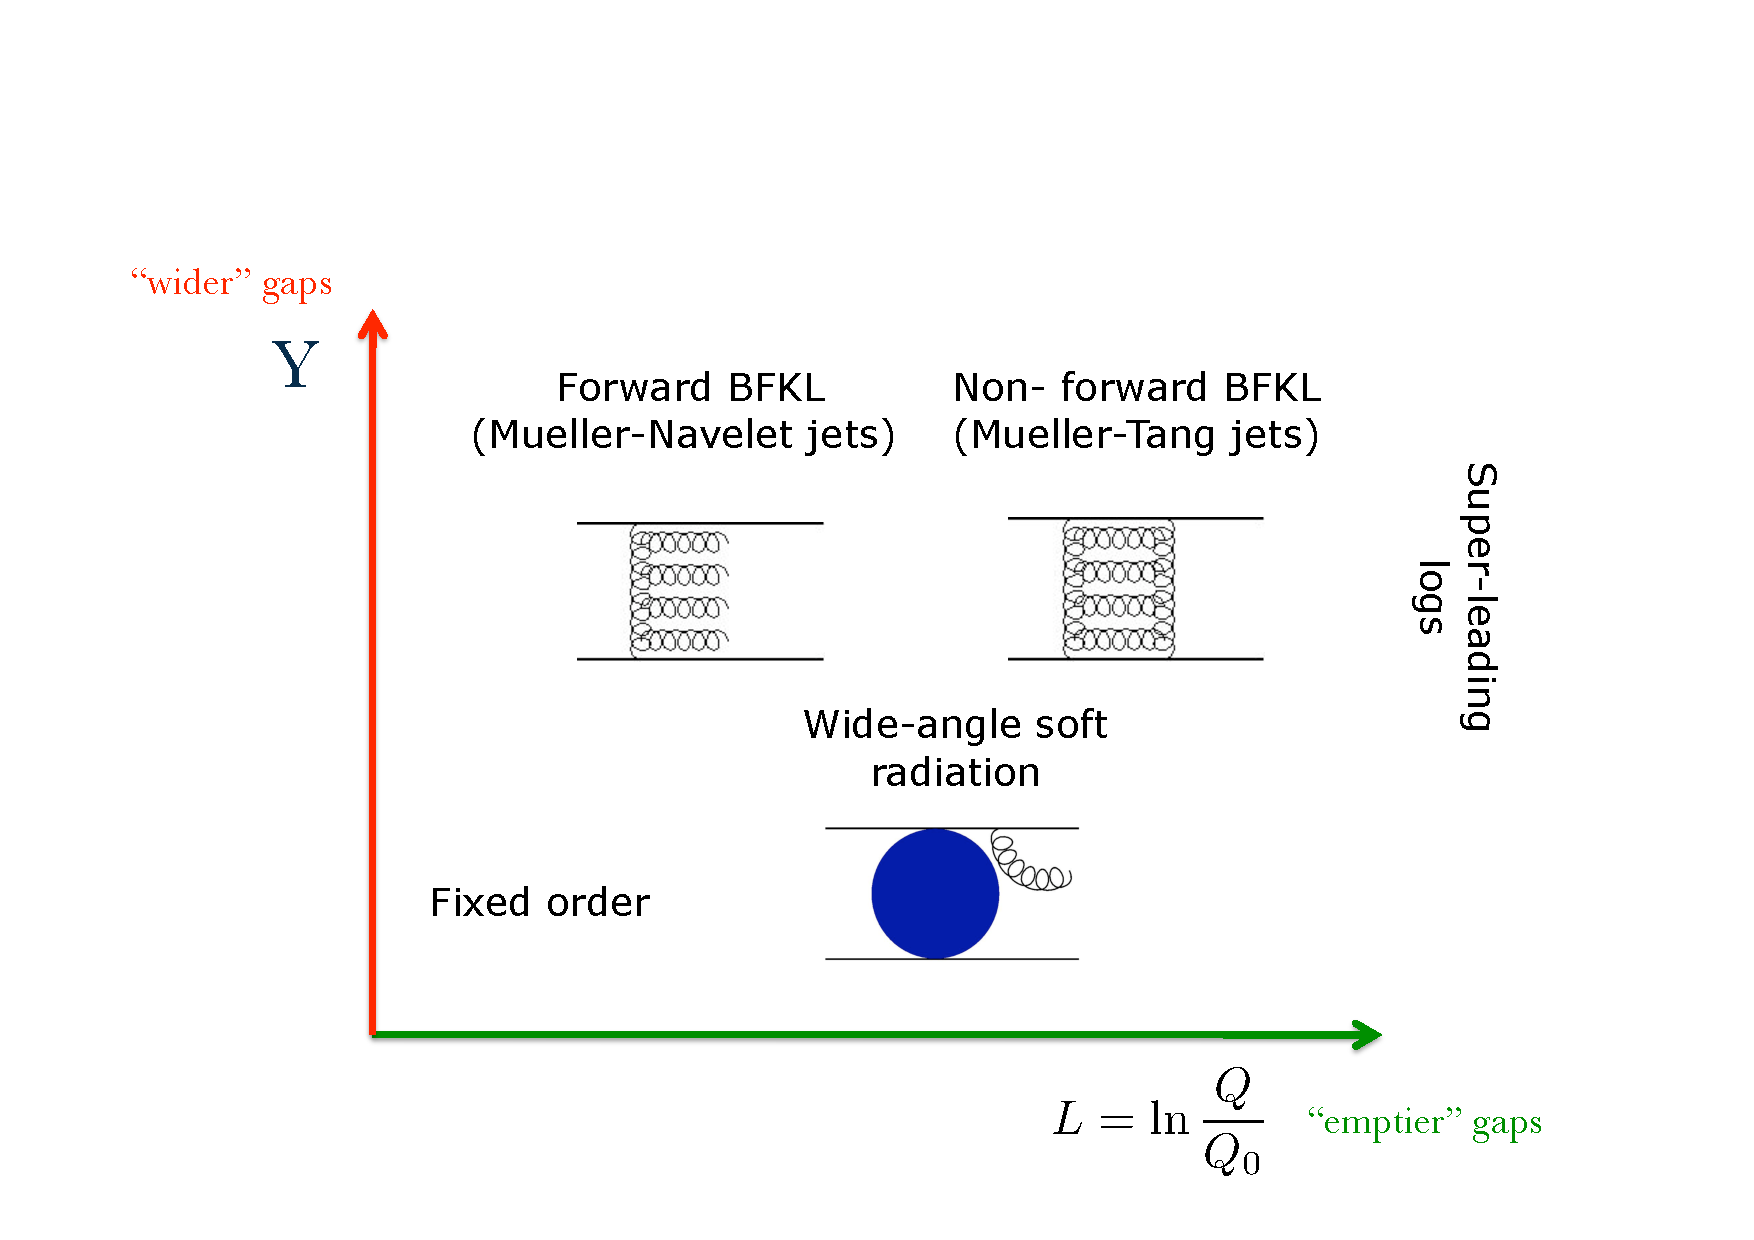
\includegraphics[width=0.8\textwidth]{figures/Theory/LY.pdf}
\caption[Illustration of the different effects on the gap fraction for a range of phase space ]{
Illustration depicting different effects that are important for the gap fraction calculation for dijet rapidity separation, Y, and $L=\ln(Q/\qz{})$.
Figure taken from \cite{ref:Forshaw_Veto}.
\label{Theory:KineRange}}
\end{figure}
%To study the emmision of radiation a veto on additional jets between the dijet can be applied.


%If an event has no jet between the dijets, it is descrived as a gap event, and 



